\documentclass{beamer}

\usepackage[T1]{fontenc}
\usepackage[polish]{babel}
\usepackage[utf8]{inputenc}
\usepackage{lmodern}
\usepackage{graphicx}
\usepackage{adjustbox} 
\usepackage{caption} 

\selectlanguage{polish}

\usetheme{Boadilla}

\setbeamertemplate{navigation symbols}{}
\setbeamertemplate{footline}{
	\leavevmode%
	\hbox{%
		% Lewa część — 0.25\textwidth
		\begin{beamercolorbox}[wd=0.25\textwidth,ht=2.5ex,dp=1.125ex,center]{author in head/foot}%
			\usebeamerfont{author in head/foot}\hspace*{2ex}\insertshortauthor
		\end{beamercolorbox}%
		% Środkowa część — 0.5\textwidth
		\begin{beamercolorbox}[wd=0.5\textwidth,ht=2.5ex,dp=1.125ex,center]{title in head/foot}%
			\usebeamerfont{title in head/foot}\insertshorttitle
		\end{beamercolorbox}%
		% Prawa część — 0.25\textwidth
		\begin{beamercolorbox}[wd=0.25\textwidth,ht=2.5ex,dp=1.125ex,center]{date in head/foot}%
			\usebeamerfont{date in head/foot}\insertframenumber{} / \inserttotalframenumber\hspace*{2ex}
		\end{beamercolorbox}%
	}%
	\vskip0pt%
}
\title{Aplikacja wspomagająca zarządzanie budżetem domowym}
\author{Dawid Ziora}
\date[]{2025}
\titlegraphic{
\includegraphics[width=0.5\linewidth]{../images/logopcz_z_logo_wiisi.png}}

\begin{document}

\maketitle

\begin{frame}{Spis treści}
	\tableofcontents
\end{frame}

\section{Prezentacja aplikacji}

\begin{frame}{\insertsection}
	\only<1>{
		\begin{block}{Formularz logowania}
			Aplikacja webowa wymaga autoryzacji.
		\end{block}
	}
	\only<2>{
	\begin{block}<2>{Tłumaczenie}
		Możliwość presonalizacji języka.
	\end{block}
	}
	\begin{columns}
		\column{0.5\textwidth} 
		\begin{figure}
			\centering
			\includegraphics[width=1\linewidth]{../images/login.png}
		\end{figure}
		\column{0.5\textwidth} 
		\begin{figure}
			\centering
			\includegraphics[width=1\linewidth]{../images/loginang.png}
		\end{figure}
	\end{columns}
\end{frame}

\begin{frame}{\insertsection}
	\begin{columns}
		\column{0.5\textwidth} 
		\begin{block}{Formularz rejestracji}
			Istnieje możliwość utworzenia konta.
		\end{block}
		\column{0.5\textwidth} 
		\begin{figure}
			\centering
			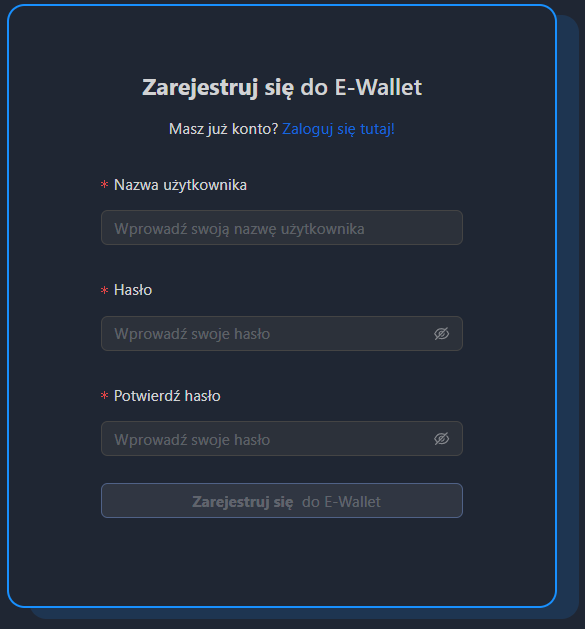
\includegraphics[width=1\linewidth]{../images/Rejestracja}
			\label{fig:rejestracja}
		\end{figure}
	\end{columns}
\end{frame}

\begin{frame}{\insertsection}
	\begin{block}{Strona główna}
		Umożliwia sprawdzanie informacji o kontach	
	\end{block}
	\begin{figure}
		\centering
		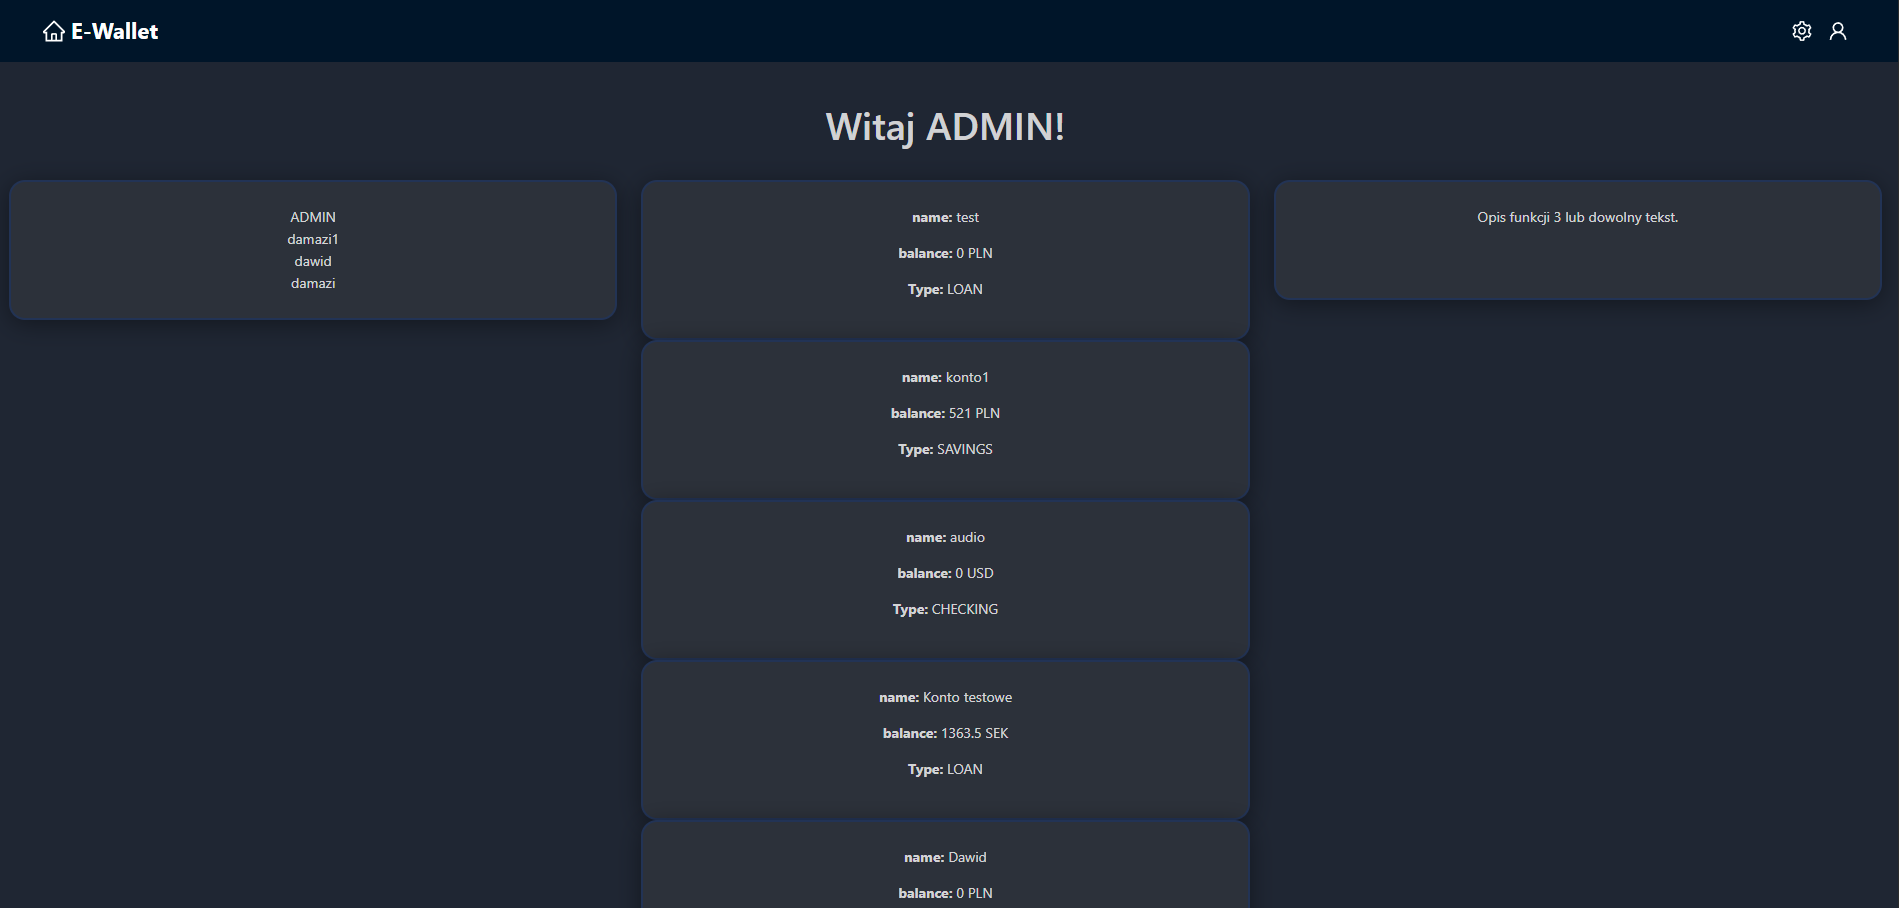
\includegraphics[width=0.9\linewidth]{../images/MotywCiemny}
	\end{figure}
\end{frame}

\begin{frame}{\insertsection}
	\begin{block}{Wybór motywu}
		Personalizacja barw aplikacji.
	\end{block}
		\begin{figure}
		\centering
		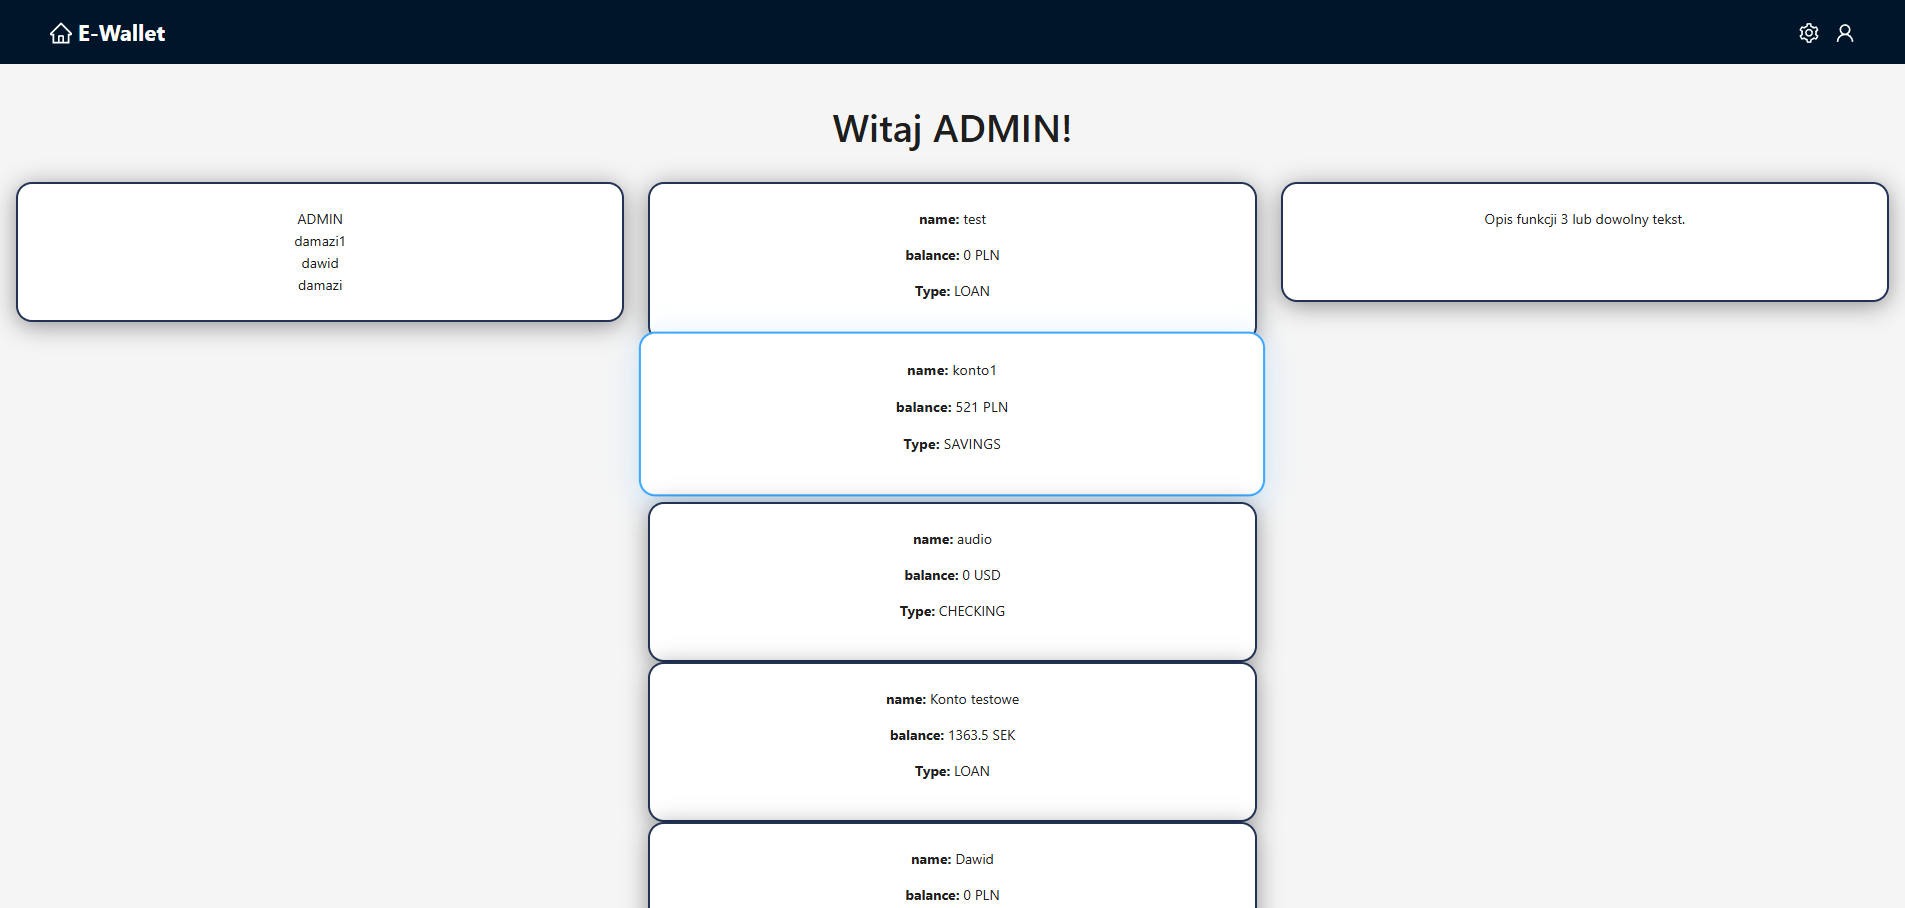
\includegraphics[width=0.9\linewidth]{../images/MotywJasny}
	\end{figure}
\end{frame}

\begin{frame}{\insertsection}
	\begin{columns}
		\column{0.45\textwidth} 
		\begin{block}{Pasek nawigacyjny}
			Udostępnia możliwość powrotu do strony głównej, dostęp do ustawień oraz wyświetlania danych użytkownika.
		\end{block}
		\begin{figure}
			\centering
			
\includegraphics[width=0.7\linewidth]{../images/Navbar}
			\caption{Navbar}
			\label{fig:navbar}
		\end{figure}
		\column{0.45\textwidth} 
		\begin{block}{Ustawienia}
			Pozwala na wybór języka i motywu.
		\end{block}
		\begin{figure}
			\centering
			
\includegraphics[width=0.7\linewidth]{../images/Ustawienia}
			\caption{Ustawienia}
			\label{fig:ustawienia}
		\end{figure}	
	\end{columns}
\end{frame}

\begin{frame}{\insertsection}
	\begin{block}{Detale konta}
		Udostępnia informacje o użytkowniku
	\end{block}
	\begin{figure}
		\centering
		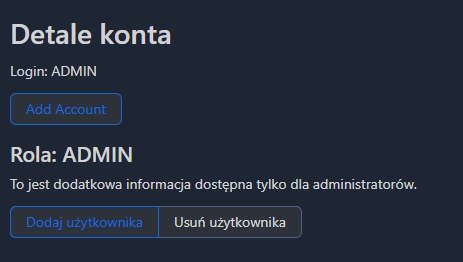
\includegraphics[width=0.7\linewidth]{../images/DetaleKonta}
		\label{fig:detalekonta}
	\end{figure}
\end{frame}

\begin{frame}{\insertsection}
\begin{columns}[t] % kolumny wyrównane do góry
	\column{0.33\textwidth}
	% minipage o stałej wysokości (tu 4.5cm) - w środku obraz wycentrowany, podpis poniżej (na stałej pozycji)
	\begin{minipage}[t][4.5cm][c]{\linewidth}
		\centering
		\adjustbox{valign=c}{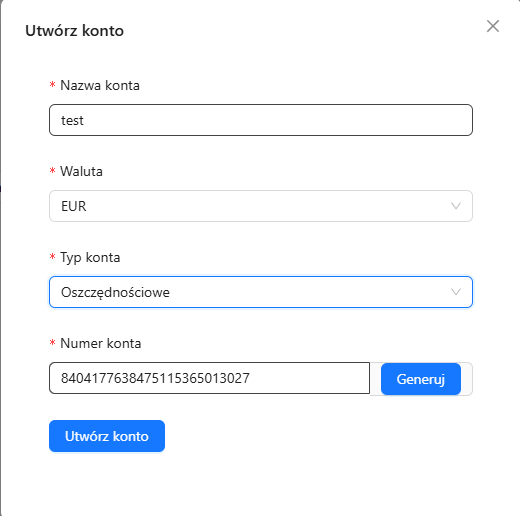
\includegraphics[width=\linewidth,keepaspectratio]{../images/AccountForm}}
	\end{minipage}
	\vspace{0.6ex}
	\captionof{figure}{Dodawanie konta}
	
	\column{0.33\textwidth}
	\begin{minipage}[t][4.5cm][c]{\linewidth}
		\centering
		\adjustbox{valign=c}{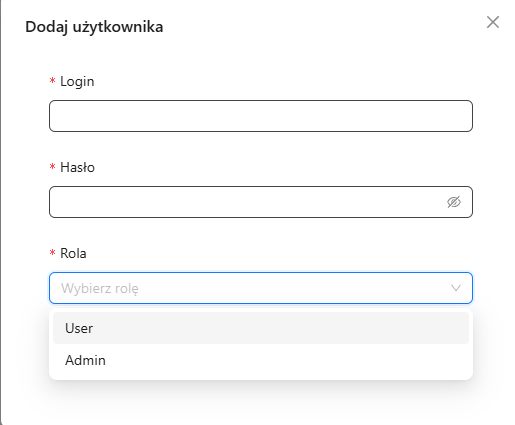
\includegraphics[width=\linewidth,keepaspectratio]{../images/DodawanieUzytkownika}}
	\end{minipage}
	\vspace{0.6ex}
	\captionof{figure}{Dodawanie użytkownika}
	
	\column{0.33\textwidth}
	\begin{minipage}[t][4.5cm][c]{\linewidth}
		\centering
		\adjustbox{valign=c}{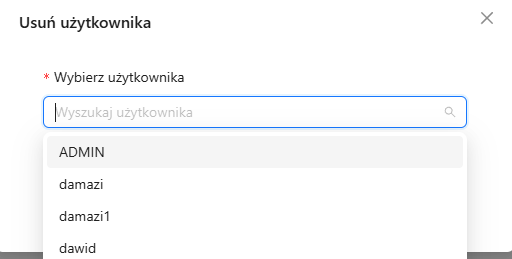
\includegraphics[width=\linewidth,keepaspectratio]{../images/UsuwanieUzytkownika}}
	\end{minipage}
	\vspace{0.6ex}
	\captionof{figure}{Usuwanie użytkownika}
\end{columns}
\end{frame}

\begin{frame}{\insertsection}
	\begin{block}{Detale portfela}
		Wyświetlanie danych o wpłatach i wypłatach.
	\end{block}
	\begin{columns}
		\column{0.45\textwidth}
			\begin{figure}
			\centering
			
\includegraphics[width=1\linewidth]{../images/DanePortfela}
			\label{fig:daneportfela}
		\end{figure}
		\column{0.45\textwidth}
		\begin{figure}
			\centering
			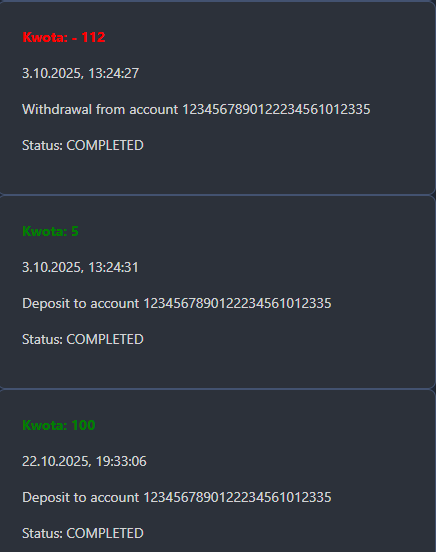
\includegraphics[width=0.9\linewidth]{../images/TransakcjeHistoria}
			\label{fig:transakcjehistoria}
		\end{figure}
		
	\end{columns}

\end{frame}

\begin{frame}{\insertsection}
\begin{figure}
	\centering
	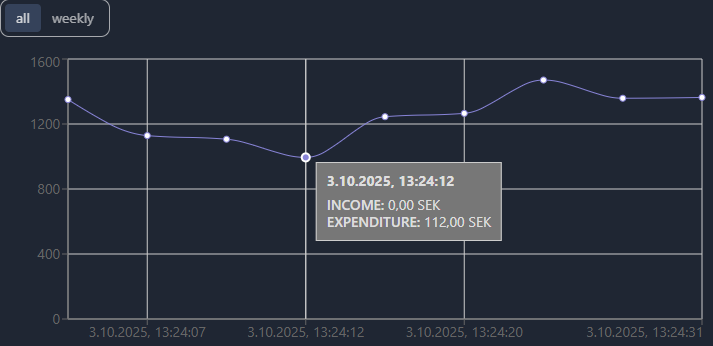
\includegraphics[width=1\linewidth]{../images/TransakcjeAll}
	\caption{Wszystkie wpłaty i wypłaty}
	\label{fig:transakcjeall}
\end{figure}
\end{frame}

\begin{frame}{\insertsection}
\begin{figure}
	\centering
	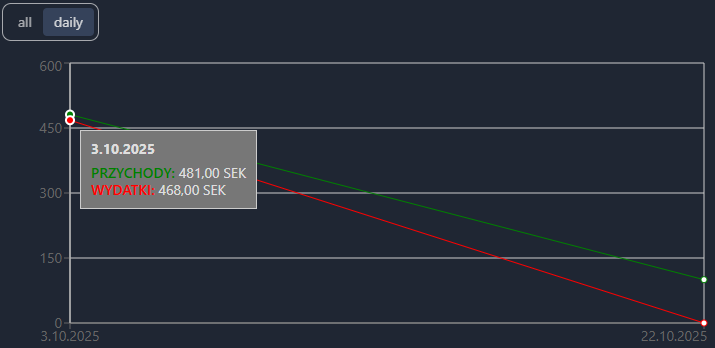
\includegraphics[width=1\linewidth]{../images/TransakcjeDaily}
	\caption{Wpłaty i wypłaty za poszczególne dni}
	\label{fig:transakcjedaily}
\end{figure}
\end{frame}

\section{Technologie}
\begin{frame}{\insertsection}
	\begin{block}{Architektura klient-serwer}
		Pozwala określić komunikację między klientem, a serwerem.
	\end{block}
	\begin{figure}
		\centering
		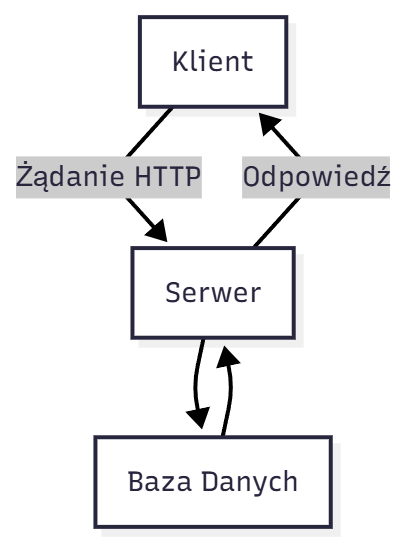
\includegraphics[height=6cm,width=0.5\linewidth]{../images/Klient-Serwer}
		\label{fig:klient-serwer}
	\end{figure}
\end{frame}

\begin{frame}{\insertsection}
	\begin{block}{Java}
		 Język zapewniający ogromne możliwości.
	\end{block}
\begin{figure}
	\centering
	
\includegraphics[width=0.9\linewidth]{../images/javaLogo}
	\label{fig:javalogo}
\end{figure}
\end{frame}

\begin{frame}{\insertsection}
	\begin{block}{Spring Boot}
		Upraszcza tworzenie, konfigurację i uruchamianie aplikacji.
	\end{block}
	\begin{figure}
		\centering
		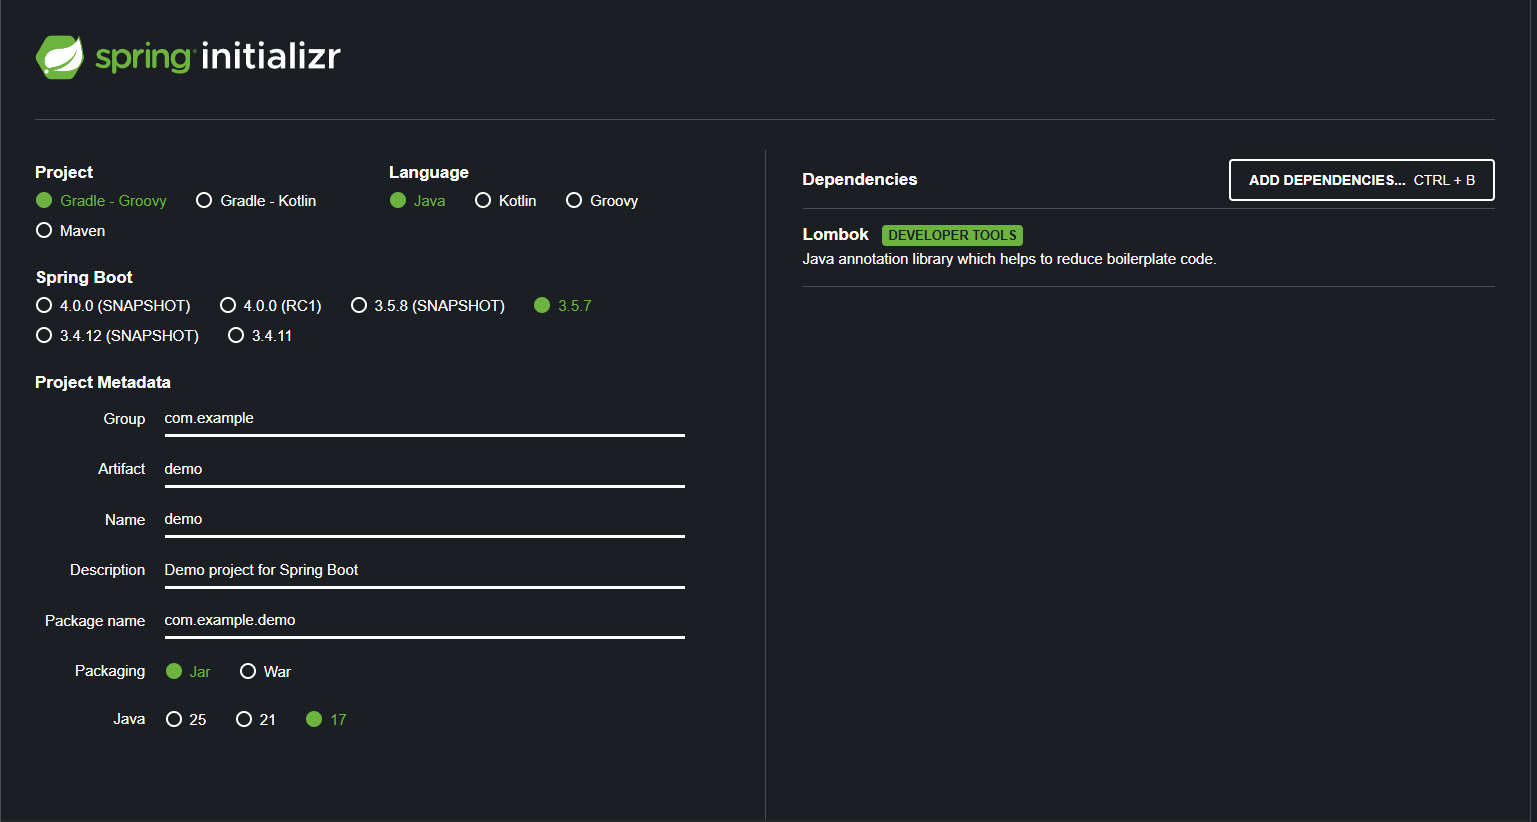
\includegraphics[width=0.9\linewidth]{../images/springInit}
		\label{fig:springinit}
	\end{figure}
\end{frame}

\begin{frame}{\insertsection}
	\begin{block}{Maven}
		Zarządzanie projektem.
	\end{block}
	\begin{figure}
		\centering
		
\includegraphics[width=0.9\linewidth]{../images/MavenLogo}
		\label{fig:mavenlogo}
	\end{figure}
\end{frame}

\begin{frame}{\insertsection}
	\begin{columns}
		\column{0.45\textwidth}
		\begin{minipage}[t][6cm][t]{\linewidth}
			\begin{block}{React}
				Biblioteka do tworzenia aplikacji webowych.
			\end{block}
			\vfill
			\centering
			
\includegraphics[height=2.2cm,keepaspectratio]{../images/ReactIcon}
		\end{minipage}
		\column{0.45\textwidth}
	 	\begin{minipage}[t][6cm][t]{\linewidth}
			\begin{block}{Język TypeScript}
				Język umożliwiający statyczne typowanie.
			\end{block}
			\vfill
			\centering
			
\includegraphics[height=2.2cm,keepaspectratio]{../images/TypeScript}
		\end{minipage}
	\end{columns}
\end{frame}

\begin{frame}{\insertsection}
	\begin{block}{MongoDB}
		Nierelacyjna baza danych, przechowująca dane w postaci dokumentów
	\end{block}
	\begin{columns}
		\column{0.2\textwidth}
			\begin{figure}
			\centering
			
\includegraphics[width=1\linewidth]{../images/MongoLogo}
			\label{fig:mongologo}
		\end{figure}
		\column{0.75\textwidth}
			\begin{figure}
			\centering
			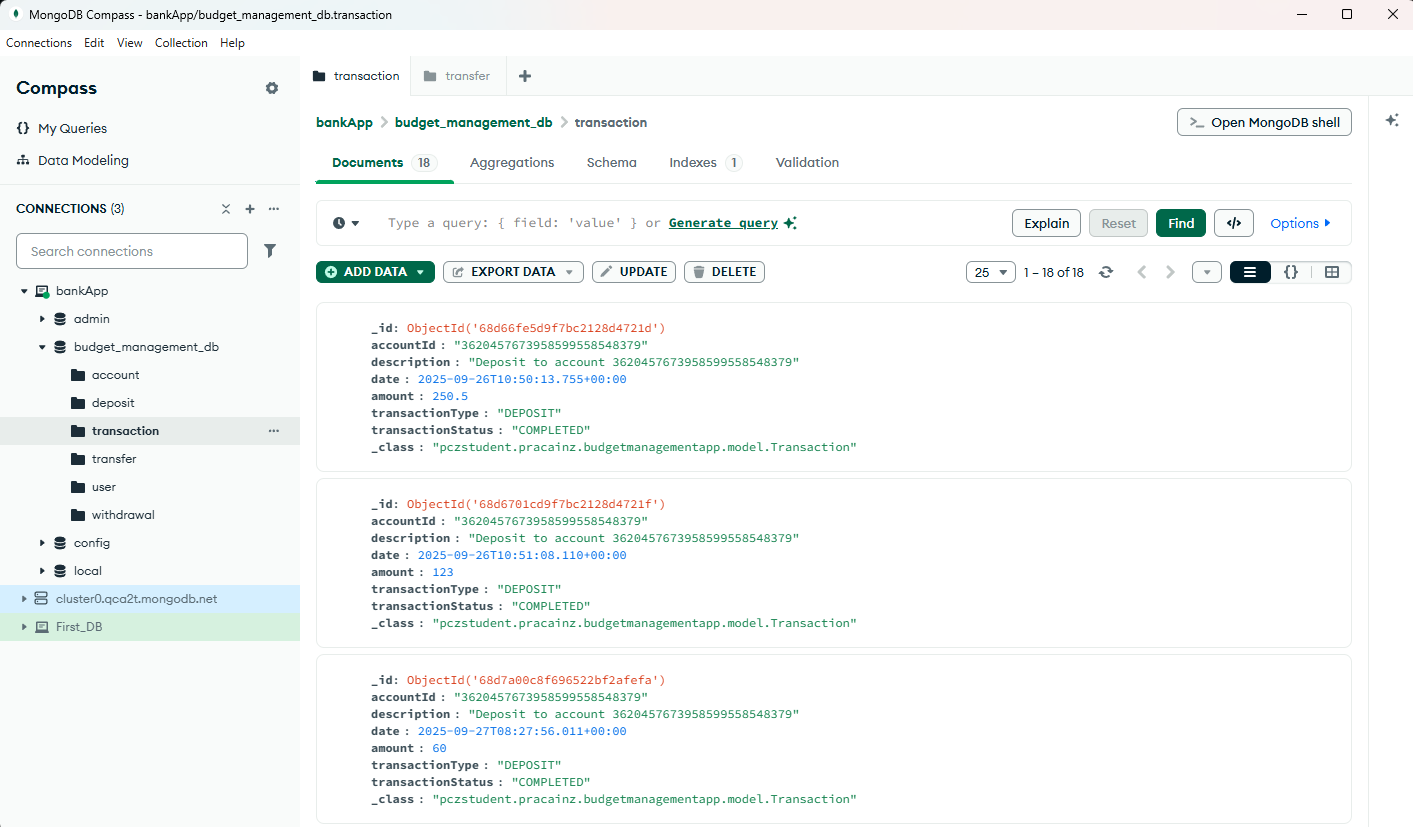
\includegraphics[width=1\linewidth]{../images/MongoData}

			\label{fig:mongodata}
		\end{figure}
	\end{columns}
\end{frame}

\section{Narzędzia}
\begin{frame}{\insertsection \space-- środowiska programistyczne}
	\begin{columns}
		\column{0.3\textwidth}
			\begin{figure}
				\centering
				
\includegraphics[width=1\linewidth]{../images/DataGrip_icon}
				\label{fig:datagripicon}
			\end{figure}		
		\column{0.3\textwidth}
			\begin{figure}
				\centering
				
\includegraphics[width=1\linewidth]{../images/IntelliJ_IDEA_icon}
				\label{fig:intellijideaicon}
			\end{figure}		
		\column{0.3\textwidth}
			\begin{figure}
				\centering
				
\includegraphics[width=1\linewidth]{../images/WebStorm_icon}
				\label{fig:webstormicon}
			\end{figure}		
	\end{columns}
\end{frame}

\begin{frame}{\insertsection}
		\begin{columns}
		\column{0.5\textwidth}
		\begin{figure}
			\centering
			\label{fig:dockerlogo}
			
\includegraphics[height=1cm,keepaspectratio]{../images/DockerLogo}
		\end{figure}
		\begin{figure}
			\centering
			
\includegraphics[height=1cm,keepaspectratio]{../images/GitLogo}
			\label{fig:gitlogo}
					\begin{figure}
				\centering
				\label{fig:junitlogo}
				
\includegraphics[height=1cm,keepaspectratio]{../images/JUnitLogo}
			\end{figure}
			\begin{figure}
				\centering
				
\includegraphics[height=1cm,keepaspectratio]{../images/PostmanLogo}
				\label{fig:postmanlogo}
			\end{figure}
			\begin{figure}
				\centering
				
\includegraphics[height=1cm,keepaspectratio]{../images/ViteLogo}
				\label{fig:vitelogo}
			\end{figure}
		\end{figure}
		\column{0.5\textwidth}
		\only<1>{\begin{block}{Docker}
			Narzędzie do konteneryzacji.
			\begin{figure}
				\centering
				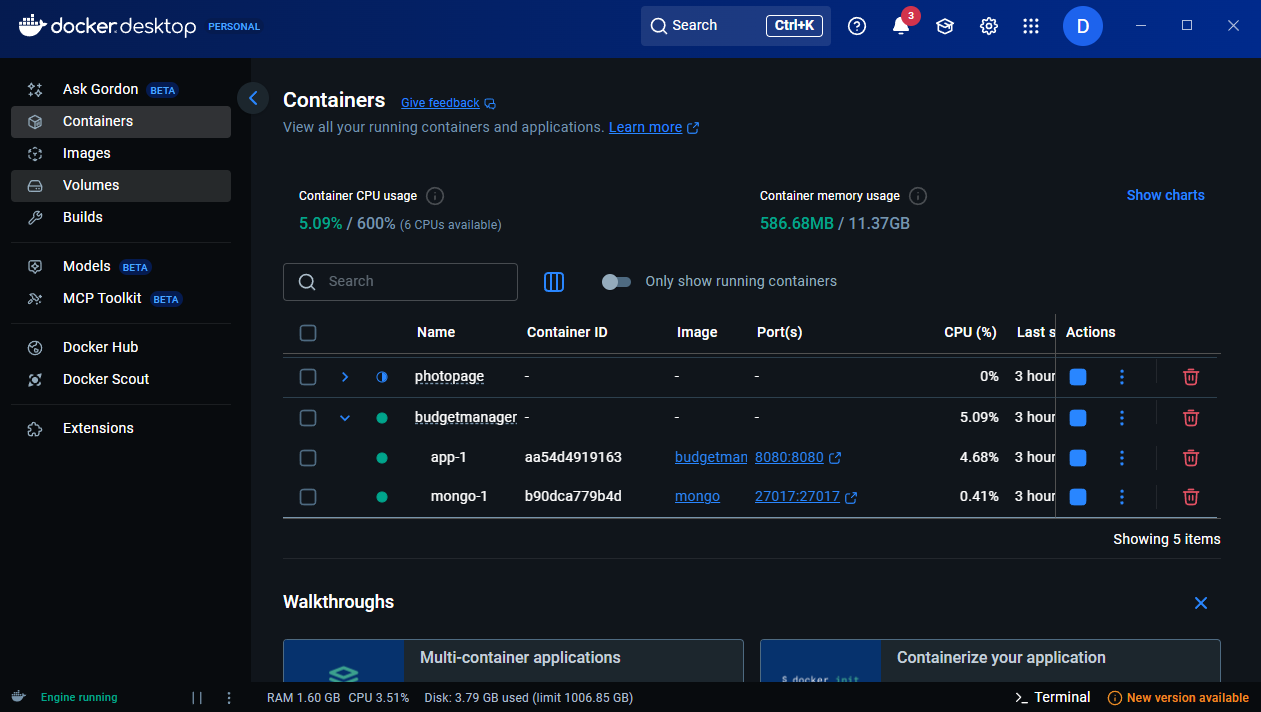
\includegraphics[width=1\linewidth]{../images/DockerApp}
				\label{fig:dockerapp}
			\end{figure}
		\end{block}
		}
		\only<2>{\begin{block}{Kontrola wersji}
			Repozytoria z możliwością zapisywania zmian w kodzie.
		\begin{figure}
			\centering
		
			\label{fig:gitlogs}
			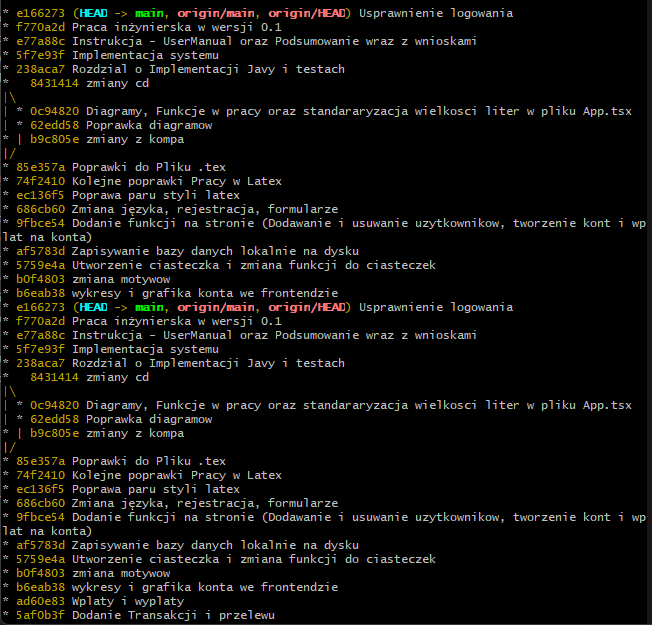
\includegraphics[width=1\linewidth]{../images/GitLogs}
		\end{figure}
		\end{block}
		}
		\only<3>{
		\begin{block}{Testy funkcjonalne}
		Sprawdzanie działania funkcji
		\begin{figure}
			\centering
			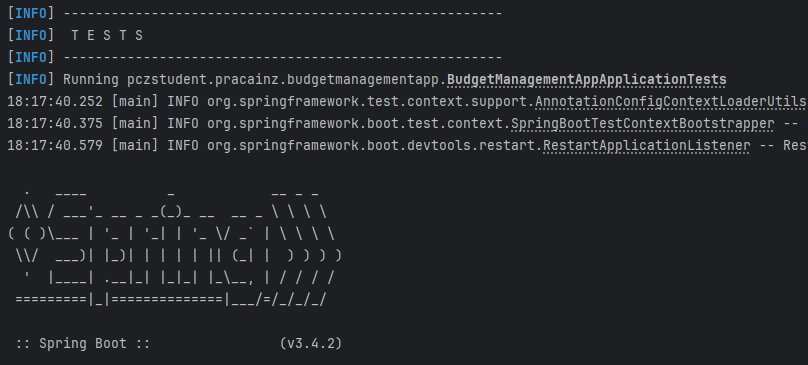
\includegraphics[width=1\linewidth]{../images/Testy}
		
			\label{fig:testy}
		\end{figure}
		\end{block}
		}
		\only<4>{
		\begin{block}{Testy komunikacji}
			Sprawdzanie odpowiedzi na żądania klienta.
		\begin{figure}
			\centering
			\label{fig:postmantest}
			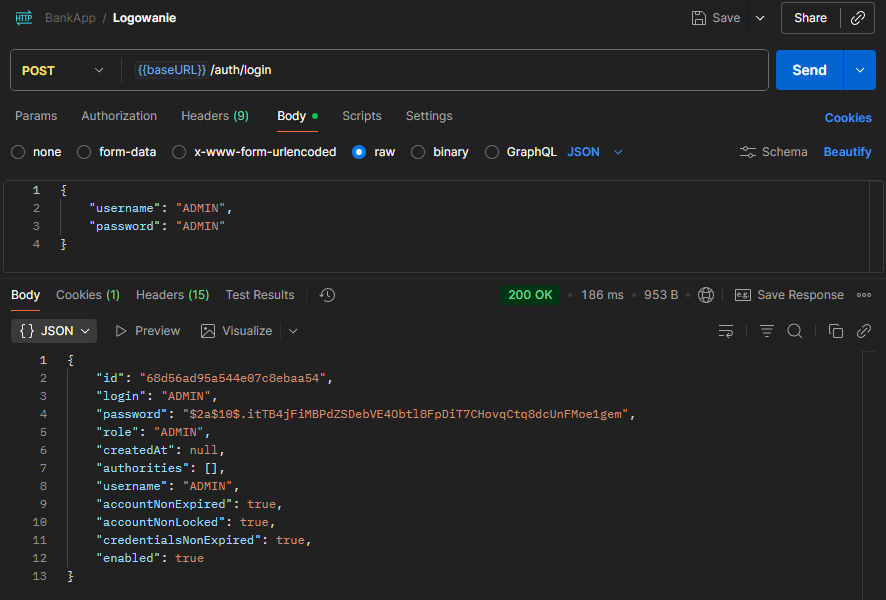
\includegraphics[width=1\linewidth]{../images/PostmanTest}
		\end{figure}
		\end{block}
		}
	\end{columns}
\end{frame}

\end{document}